\chapter{UML: Anwendungsfalldiagramm}\label{ch:uml_uc}
Eines der UML-Diagramme dieses Softwareprojektes ist das Anwendungsfalldiagramm, 
das die Interaktionen zwischen dem System und den Benutzern darstellt. 
Dabei werden Anwendungsmöglichkeiten der Software aufgezeigt, um diese zu definieren und ihre einzelnen Abhängigkeiten 
mit benötigten Aktionen und Bedingungen zu verdeutlichen.
Der Nutzer stellt in unserem Fall den Spieler dar, der sich das Spiel heruntergeladen hat und es zum ersten oder 
wiederholten Mal startet.\\
\newline
Das Anwendungsfalldiagramm teilt sich auf in den vollständigen Überblick in Abbildung~\ref{fig:uc_gesamt} und das 
Detaildiagramm in Abbildung~\ref{fig:uc_detail}.
Der vollständige Überblick zeigt grob alle Anwendungsfälle, die in unserem Projekt vorkommen,
während das Detaildiagramm die einzelnen Anwendungsfälle detaillierter darstellt. 
Im Detaildiagramm wurde der Anwendungsfall der Minispiele innerhalb des Spiels modelliert und zeigt die Anwendungsfälle,
wenn der Spieler die Minispielszene öffnet. \\

\section{Vollständiger Überblick}\label{sec:vollstandiger-uberblick}
% Beschreibung
In diesem Abschnitt wird der vollständige Überblick in Abbildung~\ref{fig:uc_gesamt} der Anwendungsfälle des Spiels 
modelliert und beschrieben.
Zu Beginn des Spiels wird der Nutzer mit dem Hauptmenü begrüßt.
Von dort aus kann dieser als Akteur das Spiel starten oder lädt ein Spiel, falls er schon einmal einen Spielstand 
erstellt hat.
Zusätzlich vor dem Spielstart kann der Nutzer einen Charakter auswählen, der ihn repräsentiert. 
Beide Aktionen sind optional, da der Nutzer das Spiel zum ersten Mal starten könnte und als Standard der erste 
Charakter ausgewählt ist.\\
Innerhalb der Hauptspielszene, die das Haus des Nutzers darstellt, kann der Nutzer nun den Shop öffnen zum Kaufen 
von Pflanzen. 
Um darin eine Pflanze zu kaufen, muss die Münzenanzahl des Nutzers ausreichend sein für die gewünschte Pflanze.
Nach dem Kauf wird die Pflanze automatisch in das Haus des Nutzers transferiert.\\
Pflanzen können wie im realen Leben durch ein Anklick-Event gegossen werden.
Damit diese im Spiel nicht verrotten oder vertrocknen, sollte der Nutzer den Wasserstand seiner Pflanzen prüfen, 
bevor er ihnen zu wenig oder zu viel Wasser geben würde. 
Dies kann er in seinem Haus durchführen, jedoch erinnert das Spiel den Nutzer nicht daran, 
weswegen die Wasserstandsprüfung keine zwingende Bedingung für das Gießen der Pflanzen ist.\\
Im Haus hat der Nutzer ein Inventar und kann darüber das Aussehen der Töpfe seiner Pflanzen ändern. 
Zu Spielbeginn besitzt der Spieler eine Auswahl an einfarbigen Töpfen und keine Skins aus den Potpacks. \\ 
Als Letztes kann der Nutzer noch das Minispielmenü öffnen, worin dieser Packs öffnen und Memory spielen kann,
was genauer im Detaildiagramm~\ref{sec:detaildiagramme} erklärt und beschrieben wird.

% Diagramm
\begin{figure}[h]
    \centering
    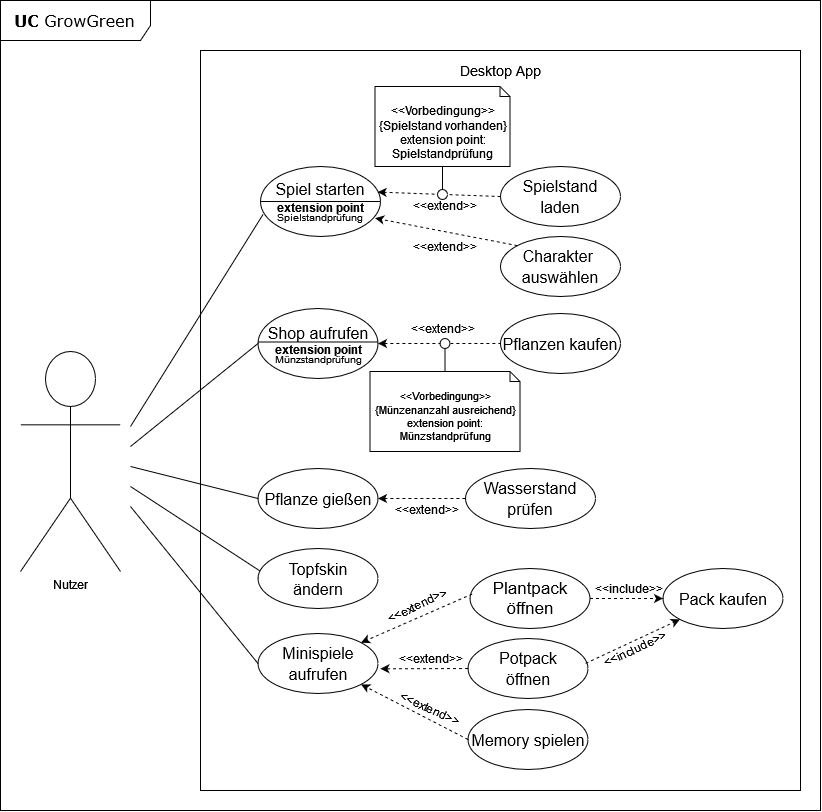
\includegraphics[width=0.8\linewidth]{../bilder/uc_gesamt}
    \vspace{0.05cm}
    \caption{Vollständiger Überblick}
    \label{fig:uc_gesamt}
\end{figure}

\newpage
\section{Detaildiagramm}\label{sec:detaildiagramme}
% Beschreibung
In diesem Abschnitt wird der Anwendungsfall der Minispiele aus Abbildung~\ref{fig:uc_detail} detailliert modelliert und 
beschrieben.
Öffnet der Nutzer die Minispielszene des Spiels, dann stehen ihm drei verschiedene Optionen zur Auswahl.\\
\newline
Die ersten zwei Möglichkeiten bestehen darin, in Plantpacks eine zufällige Pflanze oder in Potpacks einen zufälligen 
Topf zu erhalten. 
Die Pflanze wird nach Erhalt im Haus des Nutzers platziert, während der Topf im Inventar des Nutzers landet.
Nach dem Auswählen des Packs kann der Nutzer anschließend durch eine Anklickinteraktion das Pack gleichzeitig kaufen
und öffnen. 
Das bedeutet, der Nutzer kann Packs auswählen, muss sie aber nicht kaufen.
Wird das Pack aber vom Nutzer gekauft, so öffnet es sich automatisch durch die Kaufbestätigung. 
Um beide Packarten kaufen zu können, muss der Nutzer ebenfalls wie zuvor beschrieben beim Pflanzenkauf im Shop genug 
Münzen besitzen, damit die benötigte Münzanzahl abgebucht werden kann. 
Andernfalls lassen sich keine Packs öffnen.\\
\newpage
Als dritte Möglichkeit kann der Nutzer das Minispiel Memory spielen, während seine Pflanzen wachsen. 
Darüber kann der Benutzer Münzen im Spiel verdienen, um sie in Packs oder im Shop ausgeben zu können für Pflanzen und 
Töpfe.
Wurde der Menüpunkt ausgewählt ist der Nutzer nicht gezwungen, das Minispiel zu starten und könnte es auch wieder
schließen.
Sollte der Nutzer das Minispiel starten, so wird ihm eine Auswahl an Karten präsentiert, die er durch Anklicken
aufdecken kann.
Als Optionen stehen ihm noch Schwierigkeitsgrade zur Auswahl, die die Anzahl der Karten und die Gewinnhöhe an Münzen
beeinflussen.
Da aber als Standardeinstellung das einfachste Level ausgewählt ist, kann der Nutzer direkt mit dem Spiel beginnen.
Ziel des Spiels ist es, zwei gleiche Karten aufzudecken, um sie zu paaren.
Nach jedem Finden eines Paares werden beide Karten entfernt und der Nutzer kann weiter Karten aufdecken.
Hat der Nutzer alle Karten erfolgreich gepaart, erhält er eine Münzbelohnung, die automatisch seinem Münzstand
hinzugefügt wird. \\

\vspace{2cm}
% Diagramm
\begin{figure}[h]
    \centering
    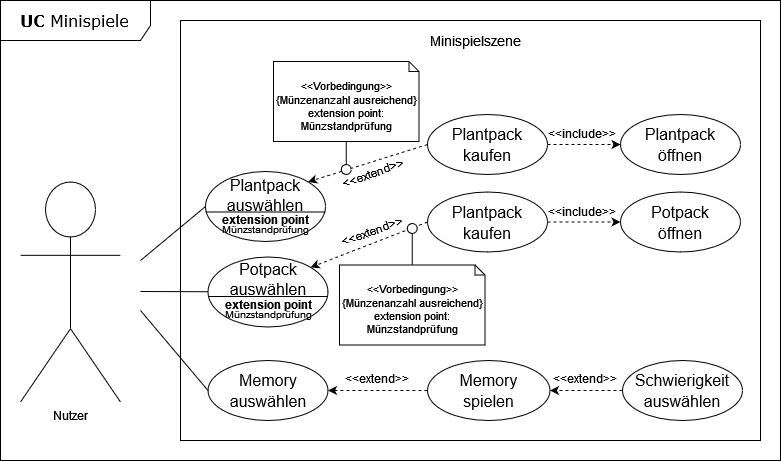
\includegraphics[width=\linewidth]{../bilder/uc_detail}
    \vspace{0.05cm}
    \caption{Detaildiagramm}
    \label{fig:uc_detail}
\end{figure}